\section{Matrix multiplication}
\label{sec:matrix_mul}

Multiplying matrices of a large size is often part of heavy scientific calculations and therefore an important building block in every mathematics library. Unfortunately, with an increasing size of the matrices the computation of the product becomes desperately slow due to an asymptotic runtime complexity of $\mathcal{O}(n^3)$ for a naive attempt. Therefore, several improvements have been tried to speed up the calculation. Strassen's algorithm for example achieves a runtime complexity of $\mathcal{O}(n^{\log_2 7}) = \mathcal{O}(n^{2.807})$ \cite{strassen} which is faster than the naive version but still does not compute results within a satisfying time for larger matrixes.
Nonetheless, modern computing systems can take advantage of one important aspect of the matrix multiplication which is it's embarrassing parallel nature. Each element of the output matrix can be computed completely independent. This potential may not only be used by today's CPU's vector extensions like SSE \footnote{Streaming SIMD Extensions, a vector instruction set extension by Intel supporting 128 bit wide registers to process 4 single precision floats in parallel.} or AVX \footnote{Advanced Vector Extensions, Intel's latest vector instruction set extension featuring 256 bit wide registers to process 8 single precision floats in parallel.}. Especially a GPU can make excellent use of the large number of independent pieces of work to perfectly utilize its hundreds or thousands of cores.

Beside the implementation and optimization of the matrix multiplication on GPUs, this chapter will also introduce the reader to performance data of GPUs collected by an appropriate profiling tool (AMD's CodeXL will be used). This will allow a better understanding about an algorithm's performance and how bottlenecks can be found and eliminated. \\
The provided benchmarks were created on a notebook with medium hardware components. Details can be found in the appendix chapter \ref{sec:becnhmark_env}. Furthermore, the host code may use the utility functions \lstinline!roundToMultiple()! and \lstinline!roundToPowerOfTwo()! for aligning input data to appropriate size. Their respective definitions can be found in appendix chapter \ref{sec:utility_functions}.

\begin{figure}
\centering
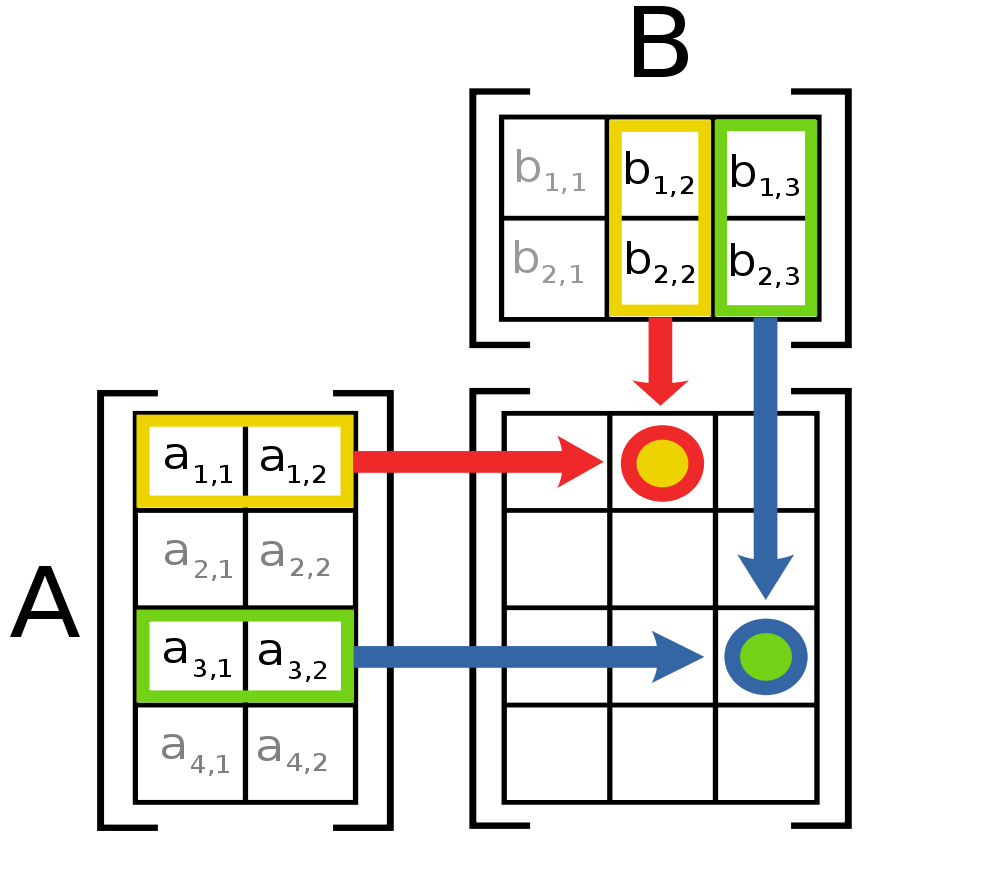
\includegraphics[width=0.5\linewidth]{matrix_mul}
\caption{Principle of the matrix multiplication \cite{wiki_matrix_mul}.}
\label{fig:matrix_mul}
\end{figure}

This chapter will take a look at different implementations of the matrix multiplication for both, the CPU and the GPU. For simplicity, square matrices are used and stored as one dimensional arrays in row major order.

\subsection{CPU Implementation}
\label{sec:matrix_cpu_implementation}

Although lots of optimized algorithms and implementations exist we will first have a look at a simple and naive implementation as the one given in listing \ref{lst:matrix_cpu}.

\lstset{basicstyle=\ttfamily{}\scriptsize{}}
\lstinputlisting[language=C++, caption=A simple C++ implementation of a square matrix multiplication for the CPU., label=lst:matrix_cpu, firstline=19, lastline=27]{code/matrix/main.cpp}
\lstset{basicstyle=\ttfamily{}}

The \lstinline!matrixMul()! function takes two pointers to the memory where the two input matrices are stored, another pointer to already allocated memory where the output is written to and a final \lstinline!n! parameter giving the edge length of the input and output matrices.
The algorithm itself is simple. Every element of the output matrix has to be calculated, therefore the outer two \lstinline!for! loops run through all of these elements. For each output element the dot product of the \lstinline!row! in matrix \lstinline!a! and the \lstinline!col! in matrix \lstinline!b! are calculated.

The performance of this implementation is conceivably slow as one can see in figure \ref{fig:matrix_chart}. Multiplying matrices with an edge length of up to 700 elements can be done in a short time (below one second), but larger matrices require a huge period of time which is unsatisfying in most cases.
Also a multithreaded version of the provided code in listing \ref{lst:matrix_cpu} (e.g. by using OpenMP and place a \lstinline!#pragma omp parallel for! above the outer for loop) does not provide a solution here, as we can see in figure \ref{fig:matrix_chart}.
The highly optimized Fortan77 BLAS library \cite{blas_lib} achieves a significant better performance when compared with the simple CPU implementation provided here.

\begin{figure}
	\centering
	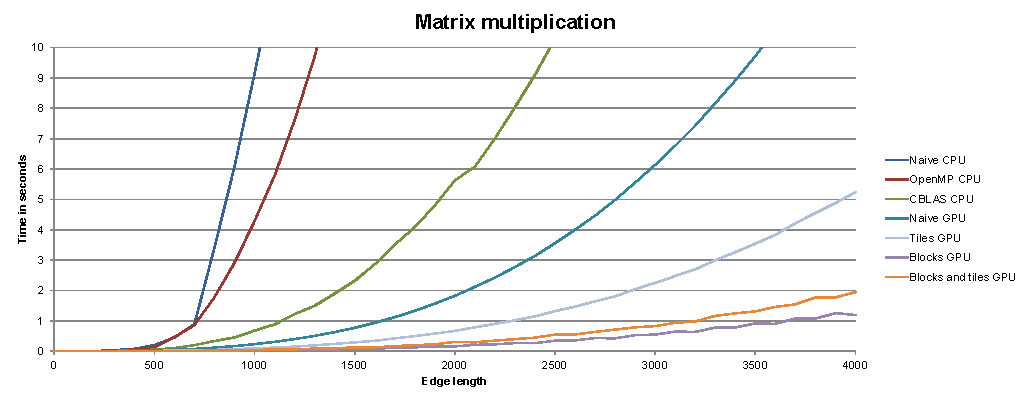
\includegraphics[width=\textwidth]{matrix_chart}
	\caption{Benchmark of several square matrix multiplication implementations. %The chart is based on the benchmark data in appendix chapter \ref{sec:matrix_mul_chart_data}.
	}
	\label{fig:matrix_chart}
\end{figure}

\subsection{Naive GPU implementation}
\label{sec:matrix_mul_naive}

A working GPU implementation can be directly derived from the simple CPU implementation given in the previous chapter \ref{sec:matrix_cpu_implementation}. As we can see in figure \ref{fig:matrix_mul}, each output element is calculated independently and the calculation of an output element corresponds to the loop body of the second \lstinline!for! loop in the CPU implementation in listing \ref{lst:matrix_cpu}. Therefore, both outer \lstinline!for! loops offering a good starting point for parallelization. 

The naive GPU implementation uses the same principle as the initial CPU version. But before we can jump into GPU code, some setup on the host is required which is given in listing \ref{lst:matrix_naive_host}. To simplify the code context and command queue have already been created and are provided as input to the \lstinline!matrixMulCL()! function.

\lstset{basicstyle=\ttfamily{}\scriptsize{}}
\lstinputlisting[language=C++, caption=Host code for a matrix multiplication implementation using OpenCL., label=lst:matrix_naive_host, firstline=29, lastline=53]{code/matrix/main.cpp}
\lstset{basicstyle=\ttfamily{}}

For the three buffers holding the two input matrices and the output matrix OpenCL buffers have to be created. On creation, additional flags may be provided to allow the underlying OpenCL implementation to optimize memory access to these buffers. Therefore, the two input matrix buffers are set to \lstinline!CL_MEM_READ_ONLY! and the output buffer is set to \lstinline!CL_MEM_WRITE_ONLY!. These flags only affect access to the memory object from the kernel code and do not restrict the host application to read or write buffers. 
After the buffers have been created, a write operation is enqueued on the command queue to the GPU for both input matrices. Note, that the third parameter of the calls to \lstinline!clEnqueueWriteBuffer()! specifies whether the function blocks until the write operation has completed or not. This parameter is set to \lstinline!false! allowing OpenCL to transfer the memory blocks asynchronously to the running host application and even in parallel .
Before the kernel can be executed, the two input buffers, the output buffer and the size of the matrix are set as arguments to the \lstinline!__kernel! function. Furthermore the global and local work size for the kernel execution have to be determined. The global work size must be a multiple of the used work group size (local work size). The chosen size of the work groups affects GPU utilization as a too small size may lead to wasted processing powers on the SMs and decreases latency tolerance. A too large work group size may cause the kernel to fill up the available register file on the SM in which case local variables are moved to global memory causing a serious drop in performance. Finding the optimal work group size is strongly hardware dependent and often boils down to simple try and error.
Note that choosing a work group size which does not evenly divide the global work size and therefor rounding the global work size to the next multiple of the work group size causes the GPU to execute the kernel for additional unneeded work items. Concerning the matrix multiplication example, the kernel would be executed for a bigger matrix with an edge length evenly dividable by the work group size. This has to be kept in mind when e.g. accessing buffers inside the kernel.
After global and local work size have been chosen, the kernel can be enqueued on the command queue to be executed by calling \lstinline!clEnqueueNDRangeKernel()!. The call immediately returns as the kernel is executed asynchronously when the command queue is flushed (\lstinline!clFlush()!) or a blocking command is enqueued, which is the case on the subsequent read operation. The call to \lstinline!clEnqueueReadBuffer()! reads the result back from the device to the host application's array. Note that the third parameter is set to \lstinline!true! indicating a blocking operation. All previously enqueued commands are ensured to be executed and finished before the read operation takes place which returns after all data has been successfully copied to client memory.

The last missing component of the naive GPU implementation is the OpenCL kernel itself which is given in listing \ref{lst:matrix_naive_kernel}.

\lstset{basicstyle=\ttfamily{}\scriptsize{}}
\lstinputlisting[language=CL, caption=OpenCL Kernel code calculating a single element of the output matrix per work item., label=lst:matrix_naive_kernel]{../src/matrix/gpu/thesis/Mult.cl}
\lstset{basicstyle=\ttfamily{}}

The \lstinline!__kernel! function closely resembles the loop body of the second \lstinline!for! loop of the CPU implementation in listing \ref{lst:matrix_cpu}. The purpose of a single invocation of this kernel is to calculate one element of the output matrix. By using OpenCL's built-in function \lstinline!get_global_id()! with the dimension as argument, the kernel invocation can retrieve it's position inside the NDRange which equals the output matrix (plus extra space due to work group size rounding). Therefore, the retrieved position has to be checked against the matrices' size as the NDRange may be larger than the original matrix. If the coordinates identify a valid matrix position, the output element is again determined by calculating the dot product of the \lstinline!row! in matrix \lstinline!a! and the \lstinline!col! in matrix \lstinline!b! and eventually written to the output matrix buffer \lstinline!c!.

When run on the GPU, the performance of this naive OpenCL implementation is already amazingly fast when we have a look at the benchmark in figure \ref{fig:matrix_chart}. At an edge length of 800 elements, the size where the CPU implementation's needed time started to blow up beyond several seconds, the GPU variant still runs very happily at around 200 milliseconds. Additionally, the curve raises far slower than the CPU's one.

However, when we have a look at the performance counters of the naive approach in table \ref{tbl:matrix_perf_counter} we notice a few things. Despite the perfect 100\% occupancy of the kernel (as a result of no local memory usage and low vector register footprint) the algorithm performs a relatively high number of fetch instructions (cf. the ALU fetch ratio of 2.5). This can also be seen at the time the fetch unit was busy, which was 99.9\%. This means the algorithm is highly memory bound. Furthermore, elements of the input matrices are accessed multiple times (edge length of output matrix times). Though this explains the nice cache behavior of 57.5\% hits, here is definitely room for improvement.
Another approach to reduce the total number of memory requests would be by querying larger elements per work item. This would lead to fewer but larger memory requests which might be handled more efficiently by the memory system. Furthermore, fewer work items would be required.

\subsection{Optimization using local memory}
\label{sec:matrix_mul_local}
Based on performance analysis of the naive GPU approach the first and most obvious optimization is to reduce the number of memory requests to global memory. Ideally, each input matrix element should be accessed only once. This scenario cannot be achieved, but the number of memory requests to a single item can be reduced to one inside smaller subregions by subdividing the input matrices into tiles as shown in figure \ref{fig:matrix_mul_local}. Instead of each work item accessing all needed input elements like in the naive version, each work item of a work group (which is equally sized as a tile) copies one element of a tile from each input matrix to local memory. After the two tiles have been copied completely, the work items than access the corresponding elements from the tiles in local memory (avoiding redundant global memory requests), multiply and add the values to the output sum of each work item (element of the output matrix). Then the next two tiles are loaded. The algorithm repeats until all tiles have been processed.

\begin{figure}
\centering
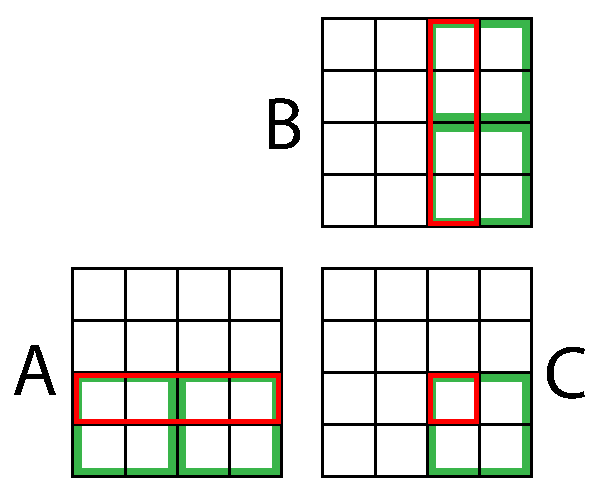
\includegraphics[width=0.5\linewidth]{matrix_mul_local}
\caption{Optimization of the matrix multiplication by subdivision into tiles.}
\label{fig:matrix_mul_local}
\end{figure}

The host code for this algorithms looks very similar to the one of the naive version. The major difference is that the edge length of the input matrix must now be a multiple of the tile size. This can be achieved by allocating slightly bigger buffers (whose edge lengths are a multiple of the tile size) and initialize them with zeros. The actual input matrices can then be copied into the upper left rectangle of the larger buffer. OpenCL offers corresponding functions to achieve this task. Listing \ref{lst:matrix_local_host} shows the host code for the optimized matrix multiplication using tiles in local memory.

\lstset{basicstyle=\ttfamily{}\scriptsize{}}
\lstinputlisting[language=CL, caption=Host code for a matrix multiplication implementation using OpenCL. The input and output matrices' edge lengths are rounded up to be a multiple of \lstinline!TILE_SIZE!., label=lst:matrix_local_host, firstline=55, lastline=95]{code/matrix/main.cpp}
\lstset{basicstyle=\ttfamily{}}

At first and most importantly a \lstinline!TILE_SIZE! hast to be defined. This parameter defines the work group size and the edge length of the square tiles that are allocated in local memory and used to cache values from global memory.
The buffers are again allocated with \lstinline!clCreateBuffer()!. If the adjusted buffer size is larger than the actual matrix size, the input buffers are initialized to zero using \lstinline!clEnqueueFillBuffer()!. Afterwards, each input matrix is copied to a rectangular region (as large as the input matrix) in the top left corner of the allocated buffer using \lstinline!clEnqueueWriteBufferRect!. For a detailed explanation of the arguments please have a look at the corresponding entry in the OpenCL specification \cite[p.76]{opencl_spec}. Apart form the kernel's arguments which equal the ones of the naive version, the work group size must be equal to the defined \lstinline!TILE_SIZE!. Finally, the results are retrieved from the output buffer following the same principle as when the inputs where copied to the input buffers.

Listing \ref{lst:matrix_local_kernel} shows the kernel code of the optimized matrix multiplication using tiles in local memory.

\lstset{basicstyle=\ttfamily{}\scriptsize{}}
\lstinputlisting[language=CL, caption=OpenCL Kernel code calculating a single element of the output matrix per wok item. The input matrixes are split into tiles which are cached in local memory. The implementation is based on J. Tompson and K. Schlachter \cite{preso}., label=lst:matrix_local_kernel,]{../src/matrix/gpu/thesis/MultLocal.cl}
\lstset{basicstyle=\ttfamily{}}

When compared with the first, naive OpenCL kernel run on the GPU, the optimization using locally cached tiles achieves a nice speedup of 2.63 at a problem size of 4000 as we can see in figure \ref{fig:matrix_chart}. % and the detailed benchmark results in appendix chapter \ref{sec:matrix_mul_chart_data}.

We can also see some improvements on the performance counters in table \ref{tbl:matrix_perf_counter}. Although the general thread management overhead remains constant (equal number of work items, work groups and therefore wave fronts) and the kernel occupancy still stays at perfect 100\% we notice a major decrease in general ALU instructions. Moreover and most importantly, fetch instructions to global memory have been reduced to a sixteenth part (due to the used \lstinline!TILE_SIZE! of 16). Despite this reduction, the eventually fetched data from global memory could only be reduced by a factor of 2.4 due to bad cache behavior.
In addition to fewer memory requests and ALU instructions a third and probably more unnoticed optimization occurred. As \lstinline!TILE_SIZE! is a compile time constant the compiler is now able to fully unroll and vectorize the inner for loop which results in more independent instructions available to the compiler to generate better filled VLIWs. This can be seen by an almost doubling of the ALU packing counter's value.


\subsection{Optimization using vectorization}
\label{sec:matrix_mul_vec}
Instead of using local memory to decrease the number of redundant memory requests this approach focuses on a better utilization of the memory system by using vector types and multiple fetches and writes per work item. Therefore, one work item does not only fetch one element but a block of elements.
The algorithm itself works conceptually equal to the local tile version of the previous chapter \ref{sec:matrix_mul_local}. The tiles are now called blocks and each work item fetches two whole blocks itself. No local memory is used, as the fetched blocks are stored in each work item's registers. Each work item then also produces an output block which is written to global memory.

The host code for this matrix multiplication version is almost identical to the one using tiles cached in local memory in listing \ref{lst:matrix_local_host}. The only differences are shown in listing \ref{lst:matrix_block_host}.

\lstset{basicstyle=\ttfamily{}\scriptsize{}}
\lstinputlisting[language=CL, caption=Differences of the host code for the matrix multiplication using vector types when compared with the one using tiles cached in local memory from listing \ref{lst:matrix_local_host}., label=lst:matrix_block_host, firstline=144, lastline=151]{code/matrix/main.cpp}
\lstset{basicstyle=\ttfamily{}}

Most importantly a \lstinline!BLOCK_SIZE! is defined, that sets the size (the edge length of a square) of the block of elements that is fetched from global memory per work item. This parameter must be one of the OpenCL supported vector type widths (which are 2, 4, 8 or 16). A larger \lstinline!BLOCK_SIZE! means more and bigger elements are fetched from global memory (better bus utilization) per work item and less work items will be needed to run the calculation (lesser thread management overhead). Furthermore, multiple independent global memory fetches can be pipelined. Additionally, as the number of elements a work item calculates increments, the number of independent instructions (instruction level parallelism) of the kernel increases allowing better ALU utilization through mostly full VLIWs (super scalar execution). However, as a consequence the required registers per work item rise which allow fewer work groups to run concurrently on a SM. For further reading Vasily Volkov from the University of California, Berkeley held a great talk about these kind of optimizations \cite{volkov}.
The determination of the optimal \lstinline!BLOCK_SIZE! is probably different for various GPUs and subject to corresponding benchmarks. The following implementation will use a value of 4.
 
Listing \ref{lst:matrix_block_kernel} shows the kernel code of the optimized matrix multiplication using vector types and multiple reads/writes to global memory per work item.

\lstset{basicstyle=\ttfamily{}\scriptsize{}}
\lstinputlisting[language=CL, caption=OpenCL Kernel code calculating a 4x4 block of elements of the output matrix per wok item using four float4 vectors. The input matrixes are accessed directly from global memory. The implementation is based on the matrix multiplication sample from AMD's APP SDK \cite{amd_app_sdk}., label=lst:matrix_block_kernel,]{../src/matrix/gpu/thesis/MultBlock.cl}
\lstset{basicstyle=\ttfamily{}}

\pagebreak

Compared with the naive GPU version we achieve an amazing speedup of 11.95 at a problem size of 4000 when we have a look at the chart in figure \ref{fig:matrix_chart}. % and the benchmark results in appendix chapter \ref{sec:matrix_mul_chart_data}.
The kernel also performs 4.54 times faster than the optimized version using locally cached tiles in chapter \ref{sec:matrix_mul_local}.

Also the performance counters in table \ref{tbl:matrix_perf_counter} show interesting changes. Most notable is the change of global work size from $4000 \times 4000$ to $1008 \times 1008$ which accounts mostly for the achieved speedup. Although the kernel now processes 16 elements instead of one, the number if needed instructions per work item only increased by a factor of 1.19 (from 20019 to 23782). Furthermore, the number of total fetch instructions per work item remained the same (a work item now issues four instructions but fetches four times more data per instruction) resulting in equal management work for the fetch unit (which is still busy at 99.4\%) but higher throughput. Additionally, as each work item processes four independent output elements, the amount of independent instructions increased leading to an almost doubling in ALU packing performance. The only major drawback of this version is that the high number of needed registers (VGPRs) limits the amount of wavefronts that can be concurrently executed on a SM. This can be seen clearly at the lower occupancy of only 37.5\%. As a result, memory latency may not be hided well enough. However, this problem is specific to the amount of available registers which increases as GPGPU computing becomes an important design factor for GPU hardware vendors.


\subsection{Combining both approaches}
The optimization attempts presented in the last two chapters \ref{sec:matrix_mul_local} and \ref{sec:matrix_mul_vec} focus on two different aspects. The first one tries to reduce the number of redundant global memory requests by subdividing the input matrices into tiles which are read once by each work group and cached in local memory. The second approach tries to improve the general memory system and ALU utilization. The final kernel presented in this chapter will combine both ideas.
As a consequence the matrices will be subdivided in two levels. On the lower level elements will be organized into small blocks which are always loaded completely by a work item. On a higher level, the blocks are then grouped together into tiles which can be cached in local memory and are always retrieved by a whole work group.

The host code for this matrix multiplication version is almost identical to the one using tiles cached in local memory in listing \ref{lst:matrix_local_host}. The only differences are shown in listing \ref{lst:matrix_block_local_host}.

\lstset{basicstyle=\ttfamily{}\scriptsize{}}
\lstinputlisting[language=CL, caption=Differences of the host code for the matrix multiplication using vector types and locally cached tiles when compared with the one using only tiles cached in local memory from listing \ref{lst:matrix_local_host}., label=lst:matrix_block_local_host, firstline=155, lastline=161]{code/matrix/main.cpp}
\lstset{basicstyle=\ttfamily{}}

The multiple of \lstinline!BLOCK_SIZE * TILE_SIZE! the matrix sizes are round up to and is required to ensure coalesced memory access and to avoid complicated bounds checking (resulting in branch divergence) inside the kernel. This value is significant higher than in the previous approaches and may account for a notable memory overhead on larger matrices (e.g. a matrix of edge length 4033 is rounded up to 4096 creating 512127 padding elements which are 3\% of the processed data).

Listing \ref{lst:matrix_block_local_kernel} shows the kernel code of the optimized matrix multiplication using vector types, multiple reads/writes to global memory per work item and locally cached tiles.

\pagebreak

\lstset{basicstyle=\ttfamily{}\scriptsize{}}
\lstinputlisting[language=CL, caption=OpenCL Kernel code calculating a 4x4 block of elements of the output matrix per work item using float4 vectors. The input matrixes are split into tiles of blocks which are cached in local memory. The implementation is based on the matrix multiplication sample from AMD's APP SDK \cite{amd_app_sdk}., label=lst:matrix_block_local_kernel,]{../src/matrix/gpu/thesis/MultBlockLocal.cl}
\lstset{basicstyle=\ttfamily{}}

Although this approach can be seen as an optimization of the block only version from chapter \ref{sec:matrix_mul_vec} by using locally cached tiles, this kernel performs, contrary to expectations, slower than the original block only version (cf. benchmark chart, figure \ref{fig:matrix_chart}). The reason for this at first glance confusing behavior is easily detected when we have a look at the corresponding performance counters in table \ref{tbl:matrix_perf_counter}.
First of all, the number of work items is equal to the block only approach and therefore also the number of resulting wavefronts the hardware has to process stays the same. The higher amount of index calculations of the kernel becomes notable in the huge increase of processed ALU instructions per work item which is almost twice as much as in the block only variant (44214 vs 23782). However, the use of local memory as a cache works successfully as can be seen at the number of fetches to global memory which has been reduced by a factor of \lstinline!TILE_SIZE! and the total number of fetched KiB which has been decreased to a fourth. So far the counter values indicate rather an increase in performance. The big penalty however comes from the high register and moreover the local memory consumption of the kernel which only allow one work group to run concurrently on a SM (the local memory usage of 32 KiB fills the entire available scratch pad memory). As a result the kernel can only run 12.5\% of the hardware supported number of wavefronts concurrently (occupancy). Memory request latency will therefore account for most of the consumed runtime. By reducing the work group size, the local memory consumption can be decreased. This would allow more wavefronts to run concurrently on the cost of more redundant global memory requests. However, this idea has not proven to be beneficial during benchmarks. Nevertheless, as hardware advances more registers and local memory will be available in the future maybe allowing this kernel to develop its full potential. 

\begin{table}
	\begin{tabular*}{\textwidth}{l @{\extracolsep{\fill}} r r r r r r r}
		Kernel         & Global size        & Work group     & Time  & Local mem & VGPRs & Occ. & Wavefronts \\
		\hline
		Mult           & $4000 \times 4000$ & $16 \times 16$ & 14390 & 0         & 6     & 100  & 84000      \\
		MultLocal      & $4000 \times 4000$ & $16 \times 16$ & 5132  & 2048      & 5     & 100  & 84000      \\
		MultBlock      & $1008 \times 1008$ & $16 \times 16$ & 1074  & 0         & 16    & 37.5 & 15914      \\
		MultBlockLocal & $1008 \times 1008$ & $16 \times 16$ & 1823  & 32768     & 31    & 12.5 & 15914      \\
	\end{tabular*}
	
	\begin{tabular*}{\textwidth}{l @{\extracolsep{\fill}} r r r r r r}
		Kernel         & ALU insts & Fetches & ALU fetch ratio & Writes & LDS fetchs & LDS writes \\
		\hline
		Mult           & 20019     & 8000    & 2.5             & 1      & 0          & 0          \\
		MultLocal      & 7767      & 500     & 15.5            & 1      & 4000       & 500        \\
		MultBlock      & 23782     & 7918    & 3.0             & 4      & 0          & 0          \\
		MultBlockLocal & 44214     & 503     & 87.9            & 4      & 18352      & 2011       \\
	\end{tabular*}
	
	\begin{tabular*}{\textwidth}{l @{\extracolsep{\fill}} r r r r r}
		Kernel         & ALU busy & ALU packing & Fetch unit busy & Cache hit & Fetch size \\
		\hline
		Mult           & 62.5     & 36.0        & 99.9            & 57.5      & 23149005   \\
		MultLocal      & 68.1     & 59.3        & 17.5            & 7.3       & 9729495    \\
		MultBlock      & 74.6     & 62.8        & 99.4            & 31.2      & 21510158   \\
		MultBlockLocal & 69.8     & 69.6        & 4.2             & 37.1      & 5030126    \\
	\end{tabular*}
	
	\vspace{\baselineskip}
	
	\begin{tabularx}{\textwidth}{>{\bfseries}l X}
		Global size &
		The global work size as specified to \lstinline!clEnqueueNDRangeKernel()!. \\
		Work group &
		The size of the work groups as specified to \lstinline!clEnqueueNDRangeKernel()!. \\
		Time &
		The time spent executing the kernel on the GPU in milliseconds. This value is measured using the on-board GPU clock. \\
		Local mem &
		The amount of local memory needed by a work group in bytes. \\
		VGPRs &
		The number of Vector General Purpose Registers needed per work item. \\
		Occ. &
		The kernel occupancy. This is an estimate of the number of in-flight wavefronts on a compute unit as a percentage of the theoretical maximum number of wavefronts that the compute unit can support. \\
		Wavefronts &
		The total number of wavefronts that where executed on all compute units. A wavefront (on an AMD GPU) is a packet of 64 hardware threads running simultaneously on a SM. \\
		ALU insts &
		The average number of ALU instructions executed per work item. \\
		Fetches &
		The average number of fetch instructions to the global memory executed per work item. \\
		Writes &
		The average number of write instructions to the global memory executed per work item. \\
		LDS fetches &
		The average number of fetch instructions to the local memory (local data share) executed per work item. \\
		LDS writes &
		The average number of write instructions to the local memory (local data share) executed per work item. \\
		ALU busy &
		The percentage of GPU time ALU instructions are processed. \\
		ALU fetch ratio &
		The ratio of ALU instructions to fetch instructions. \\
		ALU packing &
		This value indicates how well the shader compiler packs the scalar and vector instructions of the OpenCL program into 5-way VLIW instructions for the GPU. \\
		Fetch unit busy &
		The percentage of GPU time the fetch unit is busy. \\
		Cache hit &
		The percentage of fetch instructions to the global memory which could be served from the cache. \\
		Fetch size &
		The total number of kilobytes eventually fetched from global memory. \\
	\end{tabularx}
		
	\caption{Selected performance counters of all matrix multiplication kernels gathered using AMD CodeXL's GPU profiler \cite{amd_codexl}. Some values have been rounded. The descriptions of the counters are based on the tool tips provided by the CodeXL Visual Studio integration.}
	\label{tbl:matrix_perf_counter}
\end{table}

\subsection{Further implementations}
Beside the presented kernels further approaches have been implemented and benchmarked which have not been covered. However some experiences may help future developers.

\begin{description}
	\item[1D vs 2D problem dimensions] \hfill \\
	For the naive approach from chapter \ref{sec:matrix_mul_naive} it does not make a difference of the kernel is run with a 1D or 2D problem dimension. 2D seems more natural for matrices but does not affect performance.
	\item[Using images and the texture units] \hfill \\
	Using images instead of buffers as memory objects (without further specialization of access patterns) does not increase performance. Images may benefit from special hardware capabilities (e.g. texture units on a GPU provide different cache mechanisms).
	\item[Vector types vs arrays] \hfill \\
	Using vector types over an array (e.g. \lstinline!float4 a;! over \lstinline!float a[4];!) does make a difference. The blocked approach from chapter \ref{sec:matrix_mul_vec} has been implemented using arrays instead of vector types. Performance dropped by a factor of four. The reason for this is the size of a GPU's vector registers which is exactly large enough to hold a \lstinline!float4! value. Components of the vector type can only be addressed at compile time (via e.g. \lstinline!.y!). Arrays however can be addressed at runtime and therefore the compiler has to ensure that every array element is addressable. As a result an array of float values is placed into a consecutive block of registers where each element occupies only the first vector component of each register. This ensures fast array element access but on the cost of quadrupled variable size.
\end{description}

Furthermore, several libraries exist supporting GPGPU accelerated matrix multiplication.

\begin{description}
   \item[clAmdBlas \cite{cl_amd_blas}] \hfill \\
   A BLAS (Basic Linear Algebra Subprograms) library provided by AMD achieving very similar results when compared with the blocks kernel of chapter \ref{sec:matrix_mul_vec}. 
   \item[cuBlas \cite{cublas}] \hfill \\
   A BLAS (Basic Linear Algebra Subprograms) library provided by NVIDIA shipped with their CUDA Toolkit. It uses CUDA as GPU Computing language and runs on NVIDIA GPUs only.
\end{description}

\subsection{Summary and conclusion}
Multiplying matrices is an important part of many scientific applications and should therefore focus on performance. Although several extremely tuned CPU libraries have established themselves there are still very few GPU accelerated routines available. We have seen that the matrix multiplication is embarrassingly easy to implement for the GPU as the parallelism is already part of the problem's nature. However, there is still as much room for improvements on a GPU as there is on the CPU's side. By the help of profiling information (performance counters) bottlenecks of the presented implementations could be detected and tackled. We have seen the importance of avoiding redundant global memory requests by using the local memory as a programmer controlled cache. Furthermore, independent instructions are beneficial to allow for better ALU utilization by instruction level parallelism. Additionally, vector types and larger memory fetches and processed elements per work item reduce the general thread management overhead and may achieve a better utilization of the global memory subsystem. Finally, a fast GPU accelerated matrix multiplication could be implemented beating the already highly optimized BLAS library (CPU) by factor of 36 (43.49 vs 1.21 seconds)! This result definitely shows the potential of modern GPU hardware.
